% document type
\documentclass[12pt]{article}

% packages
\usepackage[total={170mm,230mm}]{geometry}
\usepackage[utf8]{inputenc}
\usepackage[T1]{fontenc}
\usepackage[russian]{babel}
\usepackage{graphicx}
\usepackage{amssymb}
\usepackage{amsfonts}
\usepackage{amsmath}
\usepackage{amsthm}
\usepackage{physics}
\usepackage{nicefrac}
\usepackage{cancel}
\usepackage{hyperref}
\usepackage{cmap}

\usepackage{multirow}

\DeclareMathOperator\sinc{sinc}

\title{Прибор Норренберга}
\author{Козлов Александр \and Краснощёкова Дарья}

\begin{document}
	\maketitle
	\section{Первая часть}
	\subsection{Изучение кристалла исландского шпата}
	\subsubsection{Определение направления главной оптической оси}
	Определили направление главной оптической оси в кристалле исландского шпата. Согласно геометрии кристаллической решётки рассматриваемого кристалла главная оптическая ось будет направлена вдоль кротчайшей пространственной диагонали ромбоэдра (см. рис. \ref{fig:1}).
	\begin{figure}[tb]
	  	\begin{center}
		\begin{minipage}[h]{0.45\linewidth}
		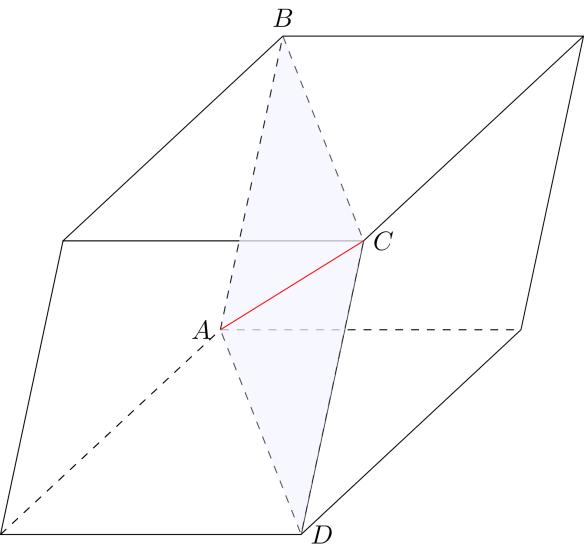
\includegraphics[width=1\linewidth]{../data/k}
		\caption{Кристалл исландского шпата, являющий собой ромбоэдр. Красным отмечена его кротчайшая диагональ.} 
		\label{fig:1}
		\end{minipage}
		\hfill
		\begin{minipage}[h]{0.45\linewidth}
		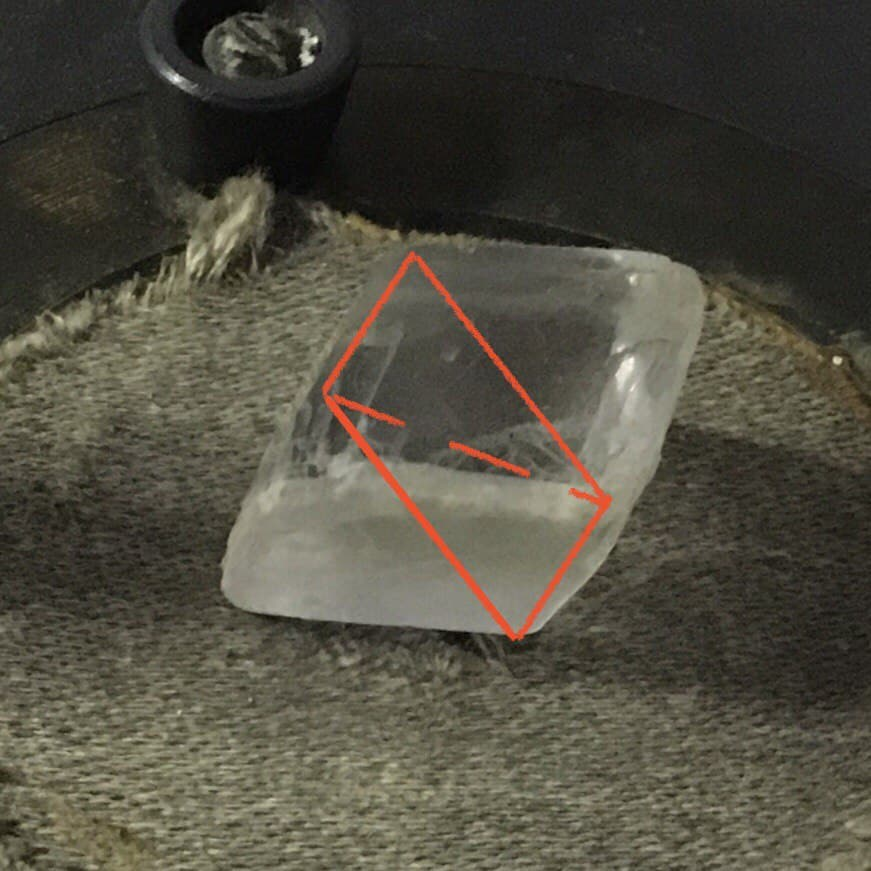
\includegraphics[width=1\linewidth]{../data/opt_ax}
		\caption{Кристалл исландского шпата, предоставленный нам для проведения эксперимента. Штрихованный отрезок обозначает направление главной оптической оси.}
		\label{fig:2}
		\end{minipage}
		\end{center}
	\end{figure}
	Отсюда нашли направление главной оптической оси кристалла (см. рис. \ref{fig:2}).

	\subsubsection{Определение плоскости главного сечения}
	Главное сечение есть плоскость, образованная главной оптической осью и вектором $\vb{k}$. Определили положение данного сечения (см. рис. \ref{fig:3}).
	\begin{figure}[tb]
		\centering
		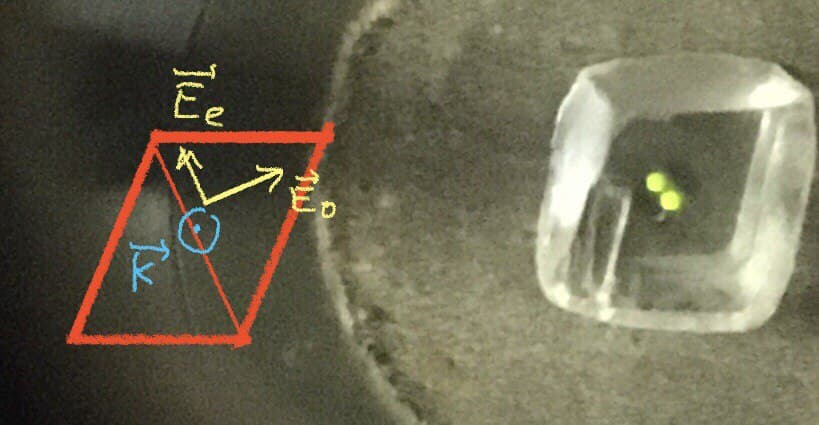
\includegraphics[width=1\linewidth]{../data/main_opt_pl}
		\caption{Наблюдение двулучепреломления в кристалле исландского шпата и определение главного сечения. Кроме того, указаны направления колебаний $\vb{E}$ в обыкновенной и необыкновенной волне.}
		\label{fig:3}
	\end{figure}

	\subsubsection{Определение плоскостей колебаний вектора $\vb{E}$ в обыкновенной и необыкновенной волне}
	В необыкновенной волне вектор $\vb{E}$ колеблется в главной плоскости, а в обыкновенной - перпендикулярно ей. Из данных соображений находим требуемые плоскости колебаний (см. рис. \ref{fig:3}).

	\subsection{Опыты с полярископом}
	\subsubsection{Двойное лучепреломление естественного света}
	Пронаблюдали двулучепреломление естественного света. Для этого рассмотрели светящиеся точки на кристалле. Точка, отвечающая обыкновенной волне, неподвижна при небольшом повороте кристалла и если убрать кристалл, остается на прежнем месте, а отвечающая необыкновенной волне смещается.
	\par Вставили в гнездо вместо наглазника анализатор и, вращая его, наблюдали за изменением яркости обеих точек. Чтобы перейти от полного гашения одной точки к полному гашению другой, анализатор нужно было повернуть на 90 градусов. Яркость точек сравнивалась при повороте на 45 градусов.

	\subsubsection{Двулучепреломление поляризованного света}
	Чтобы определить направление колебаний вектора $\vb{E}$, пропускаемых поляризатором полярископа, установили поляризатор между светодиодом и кристаллом, затем, вращая кристалл, выбрали положение, когда одна точка полностью погашена, определили какой волне соответствует данная точка. Так как мы знаем в какой плоскости колеблется вектор $\vb{E}$ для данной волны, то мы можем определять плоскость пропускания для поляризатора. Так, плоскость пропускания для обыкновенной волны перпендикулярна главному сечению, а для необыкновенной \---- параллельна главному сечению.
	\par Пронаблюдали изменение яркости обеих точек при замене наглазника анализатором. Ситуация оказалась аналогична той, которая отмечалась при наблюдении двойного преломления естественного света. Чтобы перейти от полного гашения одной точки к полному гашению другой, анализатор нужно было повернуть на 90 градусов. Чтобы яркость точек стала одинакова, анализатор нужно было повернуть на 45 градусов относительно положения, при котором одна из точек погашена.

	\section{Вторая часть}
	\subsection{Черное зеркало}
	По формуле $\tan{\varphi_\text{Б}} = n$ для $n\approx1.5$ получаем, что $\varphi_\text{Б} = 57^\circ$.
	\par Заменили стандартный анализатор черным зеркалом и установили его под углом, близким к предполагаемому углу Брюстера. Далее повернули зеркало так, чтобы достичь максимальной и минимальной интенсивности наблюдаемого белого света (положения определяли по относительной ориентировке горизонтальных осей вращения поляризующего и чёрного зеркала).
	\par Опытным путём выяснили относительную ориентировку горизонтальных осей вращения поляризующего и чёрного зеркала, при которой наблюдается максимум интенсивности белого света, нашли ориентировки и для минимума интенсивности. Когда оси были перпендикулярны, интенсивность оказывалась минимальной и была максимальна при параллельных осях (см. рис. \ref{fig:4}).
	\begin{figure}[tb]
		\centering
		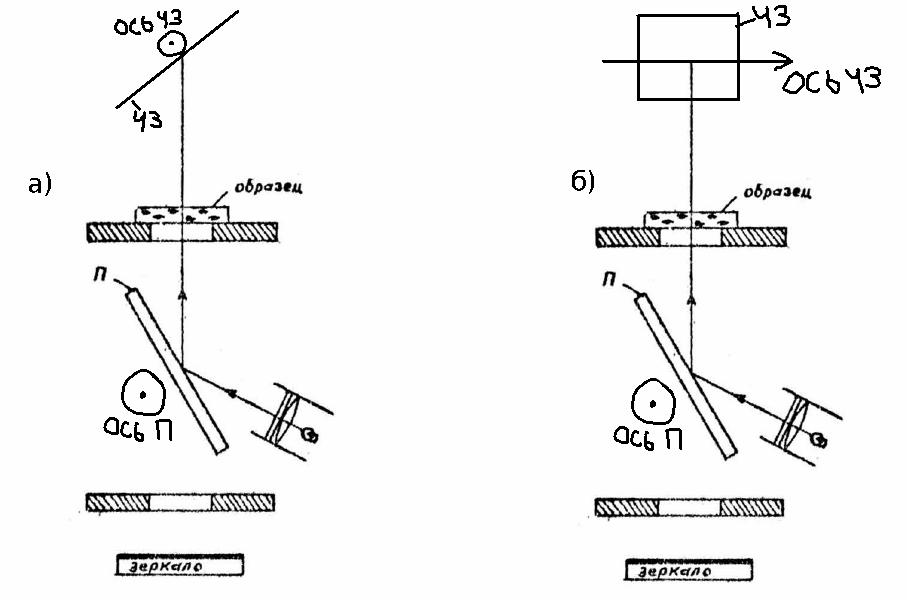
\includegraphics[width=1\linewidth]{../images/black_mirror}
		\caption{Ориентировка горизонтальных осей вращения поляризующего и чёрного зеркал. Когда оси перпендикулярны (б), интенсивность белого света минимальна, а при параллельных осях (а) \---- максимальна.}
		\label{fig:4}
	\end{figure}

	\subsection{Стопа стеклянных пластин}
	Провели ровно те же самые действия, что и для черного зеркала, для стопы стеклянных пластин. Установили, что интенсивность света, наоборот, максимальна при параллельных осях вращения поляризующего зеркала и стопы стеклянных пластин и минимальна при перпендикулярных осях.

	\subsection{Объяснение наблюдаемых явлений}
	Рассмотренные выше результаты можно объяснить следующим образом. Свет, отраженный от поляризационного зеркала, поляризован в плоскости этого зеркала. Чёрное зеркало отражает свет, поляризованный в плоскости черного зеркала. Стопа стеклянных пластин отражает свет, поляризованный в плоскости, перпендикулярной к плоскости стопы.

	\section{Третья часть}
	\subsection{Определение типа пластинок}
	Ставили анализатор на затемнение. Помещали интересующую нас пластинку на средний столик. Вращали пластинку и смотрели за изменением интенсивности картины. Если интенсивность не меняется, то оптическая ось перпендикулярна срезу. Это кварцевые пластины. Если наблюдается изменение интенсивности, то оптическая ось параллельна срезу. Это пластинки в $\lambda/2$ и $\lambda/4$. Было выявлено 2 кварцевые пластины и 3 пластины в $\lambda/2$ и $\lambda/4$.

	\subsection{Опыты с пластинками в $\lambda/2$ и $\lambda/4$}
	Поместили пластинки в $\lambda/2$ и $\lambda/4$ между скрещенными николями на среднем столике. Убедились на опыте, что гашение поля зрения происходит 4 раза за оборот, через каждые $90^\circ$. Наблюдения вели в белом свете.
	\par Из пластин с оптической осью, параллельной срезу, выявили пластины в $\lambda/2$ и $\lambda/4$. Для этого верхний анализатор поставили на затемнение, положили пластину на средний столик, выбрали светофильтр (красный/зеленый) и вращая пластину, добились затемнения верхнего анализатора. Затемнение проявляло один из лучей (обыкновенный или необыкновенный).  Далее аккуратно, стараясь не сдвинуть пластину, повернули средний столик на $45^\circ$. Вращая верхний анализатор, наблюдали за изменением интенсивности поля.
	\par Результаты наблюдений за изменением интенсивности света приведены в таблице \ref{tab:1}.
\begin{table}
\centering
\begin{tabular}{|l|l|l|l|} 
\hline
№                  & Светофильтр   & Изменение
			интенсивности & Тип
			пластины   \\ 
\hline
\multirow{3}{*}{1} & Красный       & Меняется
			очень слабо    & Не
			определено  \\ 
\cline{2-4}
                   & Зеленый       & Меняется
			очень слабо    & Не
			определено  \\ 
\cline{2-4}
                   & Белый
			свет & Меняется
			цвет           & Не
			определено  \\ 
\hline
\multirow{3}{*}{2} & Красный       & Не
			меняется             & $\lambda/4$       \\ 
\cline{2-4}
                   & Зеленый       & Меняется
			очень слабо    & Не
			определено  \\ 
\cline{2-4}
                   & Белый
			свет & Меняется
			цвет           & Не
			определено  \\ 
\hline
\multirow{3}{*}{3} & Красный       & Не
			меняется             & $\lambda/4$       \\ 
\cline{2-4}
                   & Зеленый       & Меняется
			очень слабо    & Не
			определено  \\ 
\cline{2-4}
                   & Белый
			свет & Меняется
			цвет           & Не
			определено  \\ 
\hline
\multirow{3}{*}{4} & Красный       & Меняется
			очень слабо    & Не
			определено  \\ 
\cline{2-4}
                   & Зеленый       & Меняется
			цвет           & Не
			определено  \\ 
\cline{2-4}
                   & Белый
			свет & Меняется
			цвет           & Не
			определено  \\ 
\hline
\multirow{3}{*}{5} & Красный       & Меняется
			(у половины)   & $\lambda/2$       \\ 
\cline{2-4}
                   & Зеленый       & Меняется
			(у половины)   & $\lambda/2$       \\ 
\cline{2-4}
                   & Белый
			свет & Меняется
			цвет           & Не
			определено  \\ 
\hline
\multirow{3}{*}{6} & Красный       & Меняется                   & $\lambda/2$       \\ 
\cline{2-4}
                   & Зеленый       & Меняется
			цвет           & Не
			определено  \\ 
\cline{2-4}
                   & Белый
			свет & Меняется
			цвет           & Не
			определено  \\
\hline
\end{tabular}
\caption{Таблица результатов наблюдений за изменением интенсивности света.}
\label{tab:1}
\end{table}
	
	\section{Четвёртая часть}

\end{document}